\documentclass[11pt]{article}%,twocolumn
\usepackage{url}
\usepackage{cite}
\usepackage{graphicx}
\usepackage{listings}
\usepackage{colortbl}
\usepackage{fancyvrb}
\usepackage{color}
\usepackage[ascii]{inputenc}
\usepackage{titling}
\usepackage{titlesec}
\newcommand{\subtitle}[1]{%
  \posttitle{%
    \par\end{center}
    \begin{center}\large#1\end{center}
    \vskip0.5em}%
}
\setlength{\parskip}{\baselineskip}
\titlespacing\section{0pt}{12pt plus 4pt minus 2pt}{0pt plus 2pt minus 2pt}
\titlespacing\subsection{0pt}{10pt plus 3pt minus 1pt}{0pt plus 1pt minus 1pt}
\titlespacing\subsubsection{0pt}{8pt plus 2pt minus 0pt}{0pt plus 0pt minus 0pt}

%\usepackage{appendix}

\makeatletter
\def\PY@reset{\let\PY@it=\relax \let\PY@bf=\relax%
    \let\PY@ul=\relax \let\PY@tc=\relax%
    \let\PY@bc=\relax \let\PY@ff=\relax}
\def\PY@tok#1{\csname PY@tok@#1\endcsname}
\def\PY@toks#1+{\ifx\relax#1\empty\else%
    \PY@tok{#1}\expandafter\PY@toks\fi}
\def\PY@do#1{\PY@bc{\PY@tc{\PY@ul{%
    \PY@it{\PY@bf{\PY@ff{#1}}}}}}}
\def\PY#1#2{\PY@reset\PY@toks#1+\relax+\PY@do{#2}}

\expandafter\def\csname PY@tok@gd\endcsname{\def\PY@tc##1{\textcolor[rgb]{0.63,0.00,0.00}{##1}}}
\expandafter\def\csname PY@tok@gu\endcsname{\let\PY@bf=\textbf\def\PY@tc##1{\textcolor[rgb]{0.50,0.00,0.50}{##1}}}
\expandafter\def\csname PY@tok@gt\endcsname{\def\PY@tc##1{\textcolor[rgb]{0.00,0.27,0.87}{##1}}}
\expandafter\def\csname PY@tok@gs\endcsname{\let\PY@bf=\textbf}
\expandafter\def\csname PY@tok@gr\endcsname{\def\PY@tc##1{\textcolor[rgb]{1.00,0.00,0.00}{##1}}}
\expandafter\def\csname PY@tok@cm\endcsname{\let\PY@it=\textit\def\PY@tc##1{\textcolor[rgb]{0.25,0.50,0.50}{##1}}}
\expandafter\def\csname PY@tok@vg\endcsname{\def\PY@tc##1{\textcolor[rgb]{0.10,0.09,0.49}{##1}}}
\expandafter\def\csname PY@tok@m\endcsname{\def\PY@tc##1{\textcolor[rgb]{0.40,0.40,0.40}{##1}}}
\expandafter\def\csname PY@tok@mh\endcsname{\def\PY@tc##1{\textcolor[rgb]{0.40,0.40,0.40}{##1}}}
\expandafter\def\csname PY@tok@go\endcsname{\def\PY@tc##1{\textcolor[rgb]{0.53,0.53,0.53}{##1}}}
\expandafter\def\csname PY@tok@ge\endcsname{\let\PY@it=\textit}
\expandafter\def\csname PY@tok@vc\endcsname{\def\PY@tc##1{\textcolor[rgb]{0.10,0.09,0.49}{##1}}}
\expandafter\def\csname PY@tok@il\endcsname{\def\PY@tc##1{\textcolor[rgb]{0.40,0.40,0.40}{##1}}}
\expandafter\def\csname PY@tok@cs\endcsname{\let\PY@it=\textit\def\PY@tc##1{\textcolor[rgb]{0.25,0.50,0.50}{##1}}}
\expandafter\def\csname PY@tok@cp\endcsname{\def\PY@tc##1{\textcolor[rgb]{0.74,0.48,0.00}{##1}}}
\expandafter\def\csname PY@tok@gi\endcsname{\def\PY@tc##1{\textcolor[rgb]{0.00,0.63,0.00}{##1}}}
\expandafter\def\csname PY@tok@gh\endcsname{\let\PY@bf=\textbf\def\PY@tc##1{\textcolor[rgb]{0.00,0.00,0.50}{##1}}}
\expandafter\def\csname PY@tok@ni\endcsname{\let\PY@bf=\textbf\def\PY@tc##1{\textcolor[rgb]{0.60,0.60,0.60}{##1}}}
\expandafter\def\csname PY@tok@nl\endcsname{\def\PY@tc##1{\textcolor[rgb]{0.63,0.63,0.00}{##1}}}
\expandafter\def\csname PY@tok@nn\endcsname{\let\PY@bf=\textbf\def\PY@tc##1{\textcolor[rgb]{0.00,0.00,1.00}{##1}}}
\expandafter\def\csname PY@tok@no\endcsname{\def\PY@tc##1{\textcolor[rgb]{0.53,0.00,0.00}{##1}}}
\expandafter\def\csname PY@tok@na\endcsname{\def\PY@tc##1{\textcolor[rgb]{0.49,0.56,0.16}{##1}}}
\expandafter\def\csname PY@tok@nb\endcsname{\def\PY@tc##1{\textcolor[rgb]{0.00,0.50,0.00}{##1}}}
\expandafter\def\csname PY@tok@nc\endcsname{\let\PY@bf=\textbf\def\PY@tc##1{\textcolor[rgb]{0.00,0.00,1.00}{##1}}}
\expandafter\def\csname PY@tok@nd\endcsname{\def\PY@tc##1{\textcolor[rgb]{0.67,0.13,1.00}{##1}}}
\expandafter\def\csname PY@tok@ne\endcsname{\let\PY@bf=\textbf\def\PY@tc##1{\textcolor[rgb]{0.82,0.25,0.23}{##1}}}
\expandafter\def\csname PY@tok@nf\endcsname{\def\PY@tc##1{\textcolor[rgb]{0.00,0.00,1.00}{##1}}}
\expandafter\def\csname PY@tok@si\endcsname{\let\PY@bf=\textbf\def\PY@tc##1{\textcolor[rgb]{0.73,0.40,0.53}{##1}}}
\expandafter\def\csname PY@tok@s2\endcsname{\def\PY@tc##1{\textcolor[rgb]{0.73,0.13,0.13}{##1}}}
\expandafter\def\csname PY@tok@vi\endcsname{\def\PY@tc##1{\textcolor[rgb]{0.10,0.09,0.49}{##1}}}
\expandafter\def\csname PY@tok@nt\endcsname{\let\PY@bf=\textbf\def\PY@tc##1{\textcolor[rgb]{0.00,0.50,0.00}{##1}}}
\expandafter\def\csname PY@tok@nv\endcsname{\def\PY@tc##1{\textcolor[rgb]{0.10,0.09,0.49}{##1}}}
\expandafter\def\csname PY@tok@s1\endcsname{\def\PY@tc##1{\textcolor[rgb]{0.73,0.13,0.13}{##1}}}
\expandafter\def\csname PY@tok@sh\endcsname{\def\PY@tc##1{\textcolor[rgb]{0.73,0.13,0.13}{##1}}}
\expandafter\def\csname PY@tok@sc\endcsname{\def\PY@tc##1{\textcolor[rgb]{0.73,0.13,0.13}{##1}}}
\expandafter\def\csname PY@tok@sx\endcsname{\def\PY@tc##1{\textcolor[rgb]{0.00,0.50,0.00}{##1}}}
\expandafter\def\csname PY@tok@bp\endcsname{\def\PY@tc##1{\textcolor[rgb]{0.00,0.50,0.00}{##1}}}
\expandafter\def\csname PY@tok@c1\endcsname{\let\PY@it=\textit\def\PY@tc##1{\textcolor[rgb]{0.25,0.50,0.50}{##1}}}
\expandafter\def\csname PY@tok@kc\endcsname{\let\PY@bf=\textbf\def\PY@tc##1{\textcolor[rgb]{0.00,0.50,0.00}{##1}}}
\expandafter\def\csname PY@tok@c\endcsname{\let\PY@it=\textit\def\PY@tc##1{\textcolor[rgb]{0.25,0.50,0.50}{##1}}}
\expandafter\def\csname PY@tok@mf\endcsname{\def\PY@tc##1{\textcolor[rgb]{0.40,0.40,0.40}{##1}}}
%\expandafter\def\csname PY@tok@err\endcsname{\def\PY@bc##1{\setlength{\fboxsep}{0pt}\fcolorbox[rgb]{1.00,0.00,0.00}{1,1,1}{\strut ##1}}}
\expandafter\def\csname PY@tok@kd\endcsname{\let\PY@bf=\textbf\def\PY@tc##1{\textcolor[rgb]{0.00,0.50,0.00}{##1}}}
\expandafter\def\csname PY@tok@ss\endcsname{\def\PY@tc##1{\textcolor[rgb]{0.10,0.09,0.49}{##1}}}
\expandafter\def\csname PY@tok@sr\endcsname{\def\PY@tc##1{\textcolor[rgb]{0.73,0.40,0.53}{##1}}}
\expandafter\def\csname PY@tok@mo\endcsname{\def\PY@tc##1{\textcolor[rgb]{0.40,0.40,0.40}{##1}}}
\expandafter\def\csname PY@tok@kn\endcsname{\let\PY@bf=\textbf\def\PY@tc##1{\textcolor[rgb]{0.00,0.50,0.00}{##1}}}
\expandafter\def\csname PY@tok@mi\endcsname{\def\PY@tc##1{\textcolor[rgb]{0.40,0.40,0.40}{##1}}}
\expandafter\def\csname PY@tok@gp\endcsname{\let\PY@bf=\textbf\def\PY@tc##1{\textcolor[rgb]{0.00,0.00,0.50}{##1}}}
\expandafter\def\csname PY@tok@o\endcsname{\def\PY@tc##1{\textcolor[rgb]{0.40,0.40,0.40}{##1}}}
\expandafter\def\csname PY@tok@kr\endcsname{\let\PY@bf=\textbf\def\PY@tc##1{\textcolor[rgb]{0.00,0.50,0.00}{##1}}}
\expandafter\def\csname PY@tok@s\endcsname{\def\PY@tc##1{\textcolor[rgb]{0.73,0.13,0.13}{##1}}}
\expandafter\def\csname PY@tok@kp\endcsname{\def\PY@tc##1{\textcolor[rgb]{0.00,0.50,0.00}{##1}}}
\expandafter\def\csname PY@tok@w\endcsname{\def\PY@tc##1{\textcolor[rgb]{0.73,0.73,0.73}{##1}}}
\expandafter\def\csname PY@tok@kt\endcsname{\def\PY@tc##1{\textcolor[rgb]{0.69,0.00,0.25}{##1}}}
\expandafter\def\csname PY@tok@ow\endcsname{\let\PY@bf=\textbf\def\PY@tc##1{\textcolor[rgb]{0.67,0.13,1.00}{##1}}}
\expandafter\def\csname PY@tok@sb\endcsname{\def\PY@tc##1{\textcolor[rgb]{0.73,0.13,0.13}{##1}}}
\expandafter\def\csname PY@tok@k\endcsname{\let\PY@bf=\textbf\def\PY@tc##1{\textcolor[rgb]{0.00,0.50,0.00}{##1}}}
\expandafter\def\csname PY@tok@se\endcsname{\let\PY@bf=\textbf\def\PY@tc##1{\textcolor[rgb]{0.73,0.40,0.13}{##1}}}
\expandafter\def\csname PY@tok@sd\endcsname{\let\PY@it=\textit\def\PY@tc##1{\textcolor[rgb]{0.73,0.13,0.13}{##1}}}
%\expandafter\def\csname PY@tok@err\endcsname{}

\def\PYZbs{\char`\\}
\def\PYZus{\char`\_}
\def\PYZob{\char`\{}
\def\PYZcb{\char`\}}
\def\PYZca{\char`\^}
\def\PYZam{\char`\&}
\def\PYZlt{\char`\<}
\def\PYZgt{\char`\>}
\def\PYZsh{\char`\#}
\def\PYZpc{\char`\%}
\def\PYZdl{\char`\$}
\def\PYZhy{\char`\-}
\def\PYZsq{\char`\'}
\def\PYZdq{\char`\"}
\def\PYZti{\char`\~}
% for compatibility with earlier versions
\def\PYZat{@}
\def\PYZlb{[}
\def\PYZrb{]}
\makeatother

%\pretitle{\begin{center}Master Thesis Report\\\vspace*{4 mm}\today\end{center}\vspace*{15 mm}\begin{center}}

%\posttitle{\end{center}\begin{center}\end{center}}

\begin{document}

\title{\huge Towards The Reactive Web\vspace*{15 mm}}
%\subtitle{Master Thesis Report}
\date{\today}
%\date{}
%\author{Dominic Bosch \\ Departement Mathematics and Computer Science \\ University of Basel}
\author{\fontsize{11}{9}\selectfont
Master Thesis Report\\
\vspace*{10 mm}\\
Dominic Bosch\\
Departement Mathematics and Computer Science\\
University of Basel
}
\maketitle

\renewcommand{\abstractname}{}
\begin{abstract}
\textbf{Abstract.}
t.b.d.
\end{abstract}

\section{Introduction}
t.b.d.

\begin{figure*}[htb]
%\begin{center}
\centering
%,angle=-90
  \makebox[\textwidth][c]{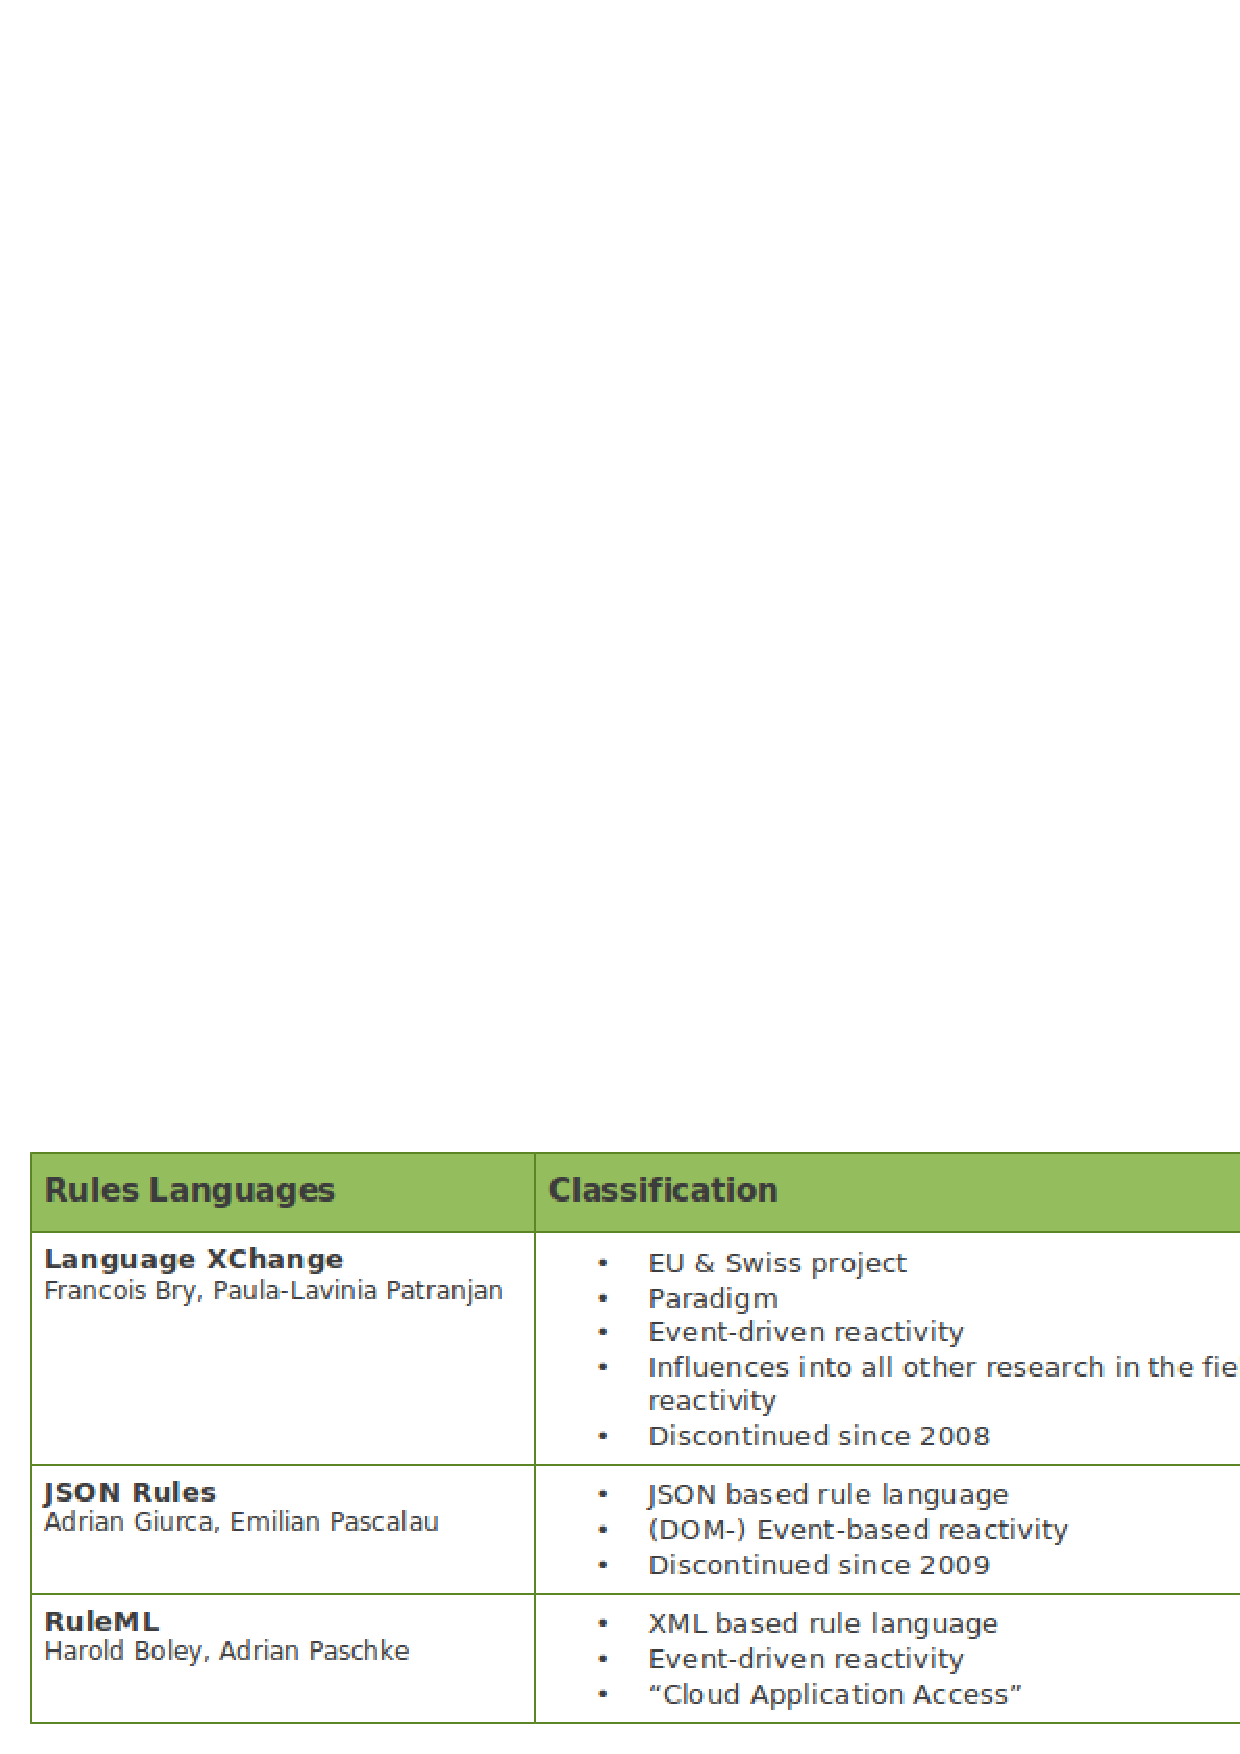
\includegraphics[scale=0.6]{img_rw_1_large}}%
\caption{Examined Rules Languages}
%\end{center}
\end{figure*}

\section{Related Work}

\subsection{Rules Languages}
\cite{2009-Paschke_Boley-RCER.pdf} gave a good oveview over existing approaches in 2009.
In this section we examine different existing rule languages with respect to a simple use case.
We want the rule language react on the receipt of an email (event), check for a distinct email address (condition) and store it in a remote location, via a Web API (action).
The email only contains the parts we require for this use case (the sender and a subject). A JSON representation of the email would be:
\begin{Verbatim}[fontsize=\small,commandchars=\\\{\}]
\PY{p}{\PYZob{}}
  \PY{l+s}{\PYZdq{}}\PY{l+s}{event}\PY{l+s}{\PYZdq{}}\PY{p}{:} \PY{l+s}{\PYZdq{}}\PY{l+s}{email}\PY{l+s}{\PYZdq{}}\PY{p}{,}
  \PY{l+s}{\PYZdq{}}\PY{l+s}{sender}\PY{l+s}{\PYZdq{}}\PY{p}{:} \PY{l+s}{\PYZdq{}}\PY{l+s}{sender@mail.com}\PY{l+s}{\PYZdq{}}\PY{p}{,}
  \PY{l+s}{\PYZdq{}}\PY{l+s}{subject}\PY{l+s}{\PYZdq{}}\PY{p}{:} \PY{l+s}{\PYZdq{}}\PY{l+s}{An important message!}\PY{l+s}{\PYZdq{}}
\PY{p}{\PYZcb{}}
\end{Verbatim}


\subsubsection{RDF \& XML}
An early ECA Rule Language for XML repositories\cite{Papamarkos03event-condition-actionrule} was postulated in 2003 and was picked up by many researches afterwards. It was designed to react on insert and delete events within XML repositories and as an action change XML documents.

\begin{Verbatim}[fontsize=\small,commandchars=\\\{\}]
\PY{n}{ON} \PY{n}{INSERT} \PY{n}{document}\PY{p}{(}\PY{l+s}{\PYZsq{}}\PY{l+s}{inbound\PYZus{}queue.xml}\PY{l+s}{\PYZsq{}}\PY{p}{)}\PY{o}{/}\PY{n}{mails}\PY{o}{/}\PY{n}{mail}
\PY{n}{IF} \PY{err}{\PYZdl{}}\PY{n}{delta}\PY{o}{/}\PY{n}{sender}\PY{p}{[}\PY{o}{.}\PY{o}{=}\PY{l+s}{\PYZsq{}}\PY{l+s}{sender@mail.com}\PY{l+s}{\PYZsq{}}\PY{p}{]}
\PY{n}{DO} \PY{n}{DELETE} \PY{n}{document}\PY{p}{(}\PY{l+s}{\PYZsq{}}\PY{l+s}{inbound\PYZus{}queue.xml}\PY{l+s}{\PYZsq{}}\PY{p}{)}\PY{o}{/}\PY{n}{mails}\PY{o}{/}\PY{n}{mail}\PY{p}{;}
   \PY{n}{LET} \PY{err}{\PYZdl{}}\PY{n}{api} \PY{o}{=} \PY{n}{resource}\PY{p}{(}\PY{l+s}{\PYZdq{}}\PY{l+s}{www.webapi.com}\PY{l+s}{\PYZdq{}}\PY{p}{)} \PY{n}{IN}
   \PY{n}{INSERT} \PY{p}{(}\PY{err}{\PYZdl{}}\PY{n}{api}\PY{p}{,} \PY{n}{newcontent}\PY{p}{,} 
      \PY{o}{\PYZlt{}}\PY{n}{content}\PY{o}{\PYZgt{}}\PY{n}{New} \PY{n}{mail}\PY{p}{:} \PY{p}{\PYZob{}}\PY{err}{\PYZdl{}}\PY{n}{delta}\PY{o}{/}\PY{n}{subject}\PY{p}{\PYZcb{}}\PY{o}{\PYZlt{}}\PY{o}{/}\PY{n}{content}\PY{o}{\PYZgt{}}\PY{p}{)}
\end{Verbatim}

Now apart from implementing a rules engine, we would also need to add an XML document event manager which interpretes and pushes events into the XML file \emph{inbound\_queue.xml}. Then again this instance would interprete the ouptuts of the ECA engine, which would theoretically manifest in other XML documents, and produce meaningful actions on remote hosts. This wouldn't be an architecture which has its focus on the solution of our use case and, as a result, add complexity and create an unnecessary overhead.

\subsubsection{Notation 3}
To make the lengthy RDF definitions smaller and more readable, Notation 3\cite{wwwn3} was designed and announced in 2005. Through the implies operator(=\textgreater) an "event" can be connected to an "action", both expressed in RDF's subject, predicate, object notation, which makes the expression of ECA rules a complicated and not very intuitive task. A solution to our use case would look as follows:

\begin{Verbatim}[fontsize=\small,commandchars=\\\{\}]
\PY{p}{\PYZob{}} \PY{err}{?}\PY{n}{x} \PY{p}{:}\PY{n}{event} \PY{l+s}{\PYZdq{}}\PY{l+s}{email}\PY{l+s}{\PYZdq{}}\PY{o}{.} \PY{err}{?}\PY{n}{x} \PY{p}{:}\PY{n}{sender} \PY{l+s}{\PYZdq{}}\PY{l+s}{sender@mail.com}\PY{l+s}{\PYZdq{}} \PY{p}{\PYZcb{}} 
    \PY{o}{=}\PY{o}{\PYZgt{}} \PY{p}{\PYZob{}} \PY{p}{:}\PY{n}{webapi} \PY{p}{:}\PY{n}{newcontent} \PY{err}{?}\PY{n}{x}\PY{p}{\PYZcb{}}
\end{Verbatim}

It's obvious that this language is used to express relations between entities and thus not really suitable for our use case, since we would require another interpreter to infer the actions. But concepts and ideas of the work that was done in these consortias could eventully still find influence into our solution.

\subsubsection{XChange/Xcerpt}
The rule language XChange\cite{2005-Patranjan-TLE.pdf} was the outcome of the REWERSE project and acted as an influence in many further researches. The language was designed to add reactive behaviour to a "static" web which is represented through XML resources. Thus we have action logics to alter such resources through insertions and deletions. Since we aim to utilize web API's for our rule language we need a more generic approach which adds flexibility in term of the API provided. But the thorough research done with the language XChange holds valuable concepts, especially in terms of temporal evet composition. This could be a rule according to our use case:

\begin{Verbatim}[fontsize=\small,commandchars=\\\{\}]
\PY{n}{TRANSACTION}
  \PY{o+ow}{in} \PY{p}{\PYZob{}} 
    \PY{n}{resource} \PY{p}{\PYZob{}} \PY{l+s}{\PYZdq{}}\PY{l+s}{http://www.webapi.com}\PY{l+s}{\PYZdq{}}\PY{p}{\PYZcb{}}\PY{p}{,}
    \PY{n}{newcontents} \PY{p}{\PYZob{}}\PY{p}{\PYZob{}}
      \PY{n}{insert} \PY{n}{newcontent} \PY{p}{\PYZob{}} \PY{n}{var} \PY{n}{Mail} \PY{p}{\PYZcb{}}
    \PY{p}{\PYZcb{}}\PY{p}{\PYZcb{}}
  \PY{p}{\PYZcb{}}
\PY{n}{ON}
  \PY{n}{xchange}\PY{p}{:}\PY{n}{event} \PY{p}{\PYZob{}}\PY{p}{\PYZob{}}
    \PY{n}{xchange}\PY{p}{:}\PY{n}{sender} \PY{p}{\PYZob{}} \PY{l+s}{\PYZdq{}}\PY{l+s}{http://mailserver.com}\PY{l+s}{\PYZdq{}} \PY{p}{\PYZcb{}}\PY{p}{,}
    \PY{n}{var} \PY{n}{Mail} \PY{o}{\PYZhy{}}\PY{o}{\PYZgt{}} \PY{n}{email} \PY{p}{\PYZob{}}\PY{p}{\PYZob{}}
      \PY{n}{sender} \PY{p}{\PYZob{}} \PY{l+s}{\PYZdq{}}\PY{l+s}{sender@mail.com}\PY{l+s}{\PYZdq{}} \PY{p}{\PYZcb{}}
    \PY{p}{\PYZcb{}}\PY{p}{\PYZcb{}}
  \PY{p}{\PYZcb{}}\PY{p}{\PYZcb{}}
\PY{n}{END}
\end{Verbatim}

But XChange is designed to access other resources in an action and thus provides powerful tools:

\begin{Verbatim}[fontsize=\small,commandchars=\\\{\}]
\PY{n}{TRANSACTION}
  \PY{p}{[}\PY{o}{.}\PY{o}{.}\PY{o}{.}\PY{p}{]}
\PY{n}{ON}
  \PY{p}{[}\PY{o}{.}\PY{o}{.}\PY{o}{.}\PY{p}{]}
\PY{n}{FROM}
  \PY{o+ow}{in} \PY{p}{\PYZob{}} 
    \PY{n}{resource} \PY{p}{\PYZob{}} \PY{l+s}{\PYZdq{}}\PY{l+s}{http://www.weather.com}\PY{l+s}{\PYZdq{}}\PY{p}{\PYZcb{}}\PY{p}{,}
    \PY{n}{temperatures} \PY{p}{\PYZob{}}\PY{p}{\PYZob{}}
      \PY{n}{var} \PY{n}{T} \PY{o}{\PYZhy{}}\PY{o}{\PYZgt{}} \PY{n}{temperature} \PY{p}{\PYZob{}}\PY{p}{\PYZob{}}
        \PY{n}{datetime} \PY{p}{\PYZob{}} \PY{l+s}{\PYZdq{}}\PY{l+s}{2013\PYZhy{}10\PYZhy{}20\PYZhy{}08:00:00AM}\PY{l+s}{\PYZdq{}} \PY{p}{\PYZcb{}}
      \PY{p}{\PYZcb{}}\PY{p}{\PYZcb{}}
    \PY{p}{\PYZcb{}}\PY{p}{\PYZcb{}}
  \PY{p}{\PYZcb{}}
\PY{n}{END}
\end{Verbatim}

\subsubsection{JSON Rules}
In 2008 \emph{JSON Rules}~\cite{2008-Giurca_Pascalau-JSON_Rules.pdf} was introduced as a language to easily react on specific DOM tree compositions.
The usage of JavaScript allowed them to provide simple functions which could be called directly by the actions, thus abstracting functionality from the language.
This key concept found influence into our language as it allows different layers of abstractions.
Through this it is possible to provide generic functions for expert user as well as very limited functions with only few possibilities for parameterization to be used by unexperienced persons.
A drawback of this language is its binding to DOM tree events, where we would want to react on any events happening in the world.
Also the temporal composition to complex events is not a subject of their work and needs further attention.

\begin{Verbatim}[fontsize=\small,commandchars=\\\{\}]
\PY{p}{\PYZob{}}
  \PY{l+s}{\PYZdq{}}\PY{l+s}{id}\PY{l+s}{\PYZdq{}}\PY{p}{:} \PY{l+m+mi}{0}\PY{p}{,}
  \PY{l+s}{\PYZdq{}}\PY{l+s}{conditions}\PY{l+s}{\PYZdq{}}\PY{p}{:} \PY{p}{[}
    \PY{p}{\PYZob{}}
      \PY{l+s}{\PYZdq{}}\PY{l+s}{type}\PY{l+s}{\PYZdq{}}\PY{p}{:} \PY{l+s}{\PYZdq{}}\PY{l+s}{email}\PY{l+s}{\PYZdq{}}\PY{p}{,}
      \PY{l+s}{\PYZdq{}}\PY{l+s}{constraints}\PY{l+s}{\PYZdq{}}\PY{p}{:} \PY{p}{[}
        \PY{p}{\PYZob{}}
          \PY{l+s}{\PYZdq{}}\PY{l+s}{propertyName}\PY{l+s}{\PYZdq{}}\PY{p}{:} \PY{l+s}{\PYZdq{}}\PY{l+s}{sender}\PY{l+s}{\PYZdq{}}\PY{p}{,}
          \PY{l+s}{\PYZdq{}}\PY{l+s}{operator}\PY{l+s}{\PYZdq{}}\PY{p}{:} \PY{l+s}{\PYZdq{}}\PY{l+s}{EQ}\PY{l+s}{\PYZdq{}}\PY{p}{,}
          \PY{l+s}{\PYZdq{}}\PY{l+s}{restriction}\PY{l+s}{\PYZdq{}}\PY{p}{:} \PY{p}{\PYZob{}}
            \PY{l+s}{\PYZdq{}}\PY{l+s}{type}\PY{l+s}{\PYZdq{}}\PY{p}{:} \PY{l+s}{\PYZdq{}}\PY{l+s}{String}\PY{l+s}{\PYZdq{}}\PY{p}{,}
            \PY{l+s}{\PYZdq{}}\PY{l+s}{value}\PY{l+s}{\PYZdq{}}\PY{p}{:} \PY{l+s}{\PYZdq{}}\PY{l+s}{sender@mail.com}\PY{l+s}{\PYZdq{}}
          \PY{p}{\PYZcb{}}
        \PY{p}{\PYZcb{}}\PY{p}{,}
        \PY{p}{\PYZob{}}
          \PY{l+s}{\PYZdq{}}\PY{l+s}{bind}\PY{l+s}{\PYZdq{}}\PY{p}{:} \PY{l+s}{\PYZdq{}}\PY{l+s}{\PYZdl{}S}\PY{l+s}{\PYZdq{}}\PY{p}{,}
          \PY{l+s}{\PYZdq{}}\PY{l+s}{propertyName}\PY{l+s}{\PYZdq{}}\PY{p}{:} \PY{l+s}{\PYZdq{}}\PY{l+s}{subject}\PY{l+s}{\PYZdq{}}
        \PY{p}{\PYZcb{}}
      \PY{p}{]}
    \PY{p}{\PYZcb{}}
  \PY{p}{]}\PY{p}{,}
  \PY{l+s}{\PYZdq{}}\PY{l+s}{actions}\PY{l+s}{\PYZdq{}}\PY{p}{:} \PY{p}{[}
    \PY{p}{\PYZob{}}
      \PY{l+s}{\PYZdq{}}\PY{l+s}{webapi(}\PY{l+s}{\PYZsq{}}\PY{l+s}{addcontent}\PY{l+s}{\PYZsq{}}\PY{l+s}{, \PYZdl{}S)}\PY{l+s}{\PYZdq{}}
    \PY{p}{\PYZcb{}}
  \PY{p}{]}
\PY{p}{\PYZcb{}}
\end{Verbatim}

\subsubsection{(Reaction) RuleML}
The basis of \emph{RuleML}~\cite{2006-Boley-RuleML.pdf} is datalog, a language in the intersection of SQL and Prolog.
In 2012 the \emph{Reaction RuleML}~\cite{2012-Paschke_etal-ReactionRuleML.pdf} language incorporated several different types of rules into the RuleML syntax, to establish a uniform syntax and interchangability of rules.
\emph{Reaction RuleML} is a valuable resource in terms of manifold research that has been done in the domain of rule languages, but the syntax is not user-friendly.


R2ML allows usage for RuleML together with many other dialects. Really!?


\subsubsection{ETALIS}
ETALIS~\cite{anicic2010arlfcepar} allows powerful temporal composition of events.

\subsubsection{KRL}
\cite{bookTheLiveWeb}
t.b.d.


\section{Conclusion}
Most of the examined rule languages are designed for the interchangability of rules between different service providers. We do not attempt to jump into this domain but we rather pick up important concepts to manifest web API's as first class citizens of our rule language. This allows the ad-hoc design and implementation of reactive rules between existing web API's without the need for their cooperation in setting up their endpoint in a special way.

\section{Future Work}
t.b.d.

\bibliography{thesisbib}
\bibliographystyle{thesisbst}

\newpage
\appendix
\lstset { basicstyle=\tiny }

\section*{Appendix}
t.b.d.
\section{ECA Rules Engine Resources}
\subsection{Node.js Rules Engine Code}
\subsubsection{ecaserver.js}

\begin{Verbatim}[fontsize=\small,commandchars=\\\{\}]
\PY{l+s}{\PYZsq{}}\PY{l+s}{use strict}\PY{l+s}{\PYZsq{}}\PY{p}{;}
\PY{n}{var} \PY{n}{express} \PY{o}{=} \PY{n}{require}\PY{p}{(}\PY{l+s}{\PYZsq{}}\PY{l+s}{express}\PY{l+s}{\PYZsq{}}\PY{p}{)}\PY{p}{;}
\PY{n}{var} \PY{n}{qs} \PY{o}{=} \PY{n}{require}\PY{p}{(}\PY{l+s}{\PYZsq{}}\PY{l+s}{querystring}\PY{l+s}{\PYZsq{}}\PY{p}{)}\PY{p}{;}
\PY{n}{var} \PY{n}{engine} \PY{o}{=} \PY{n}{require}\PY{p}{(}\PY{l+s}{\PYZsq{}}\PY{l+s}{./ecainference}\PY{l+s}{\PYZsq{}}\PY{p}{)}\PY{p}{;}
\end{Verbatim}

\end{document}
